\documentclass[12pt]{article}
\usepackage[polish]{babel}
\usepackage[utf8]{inputenc}
\usepackage{tikz}
\usetikzlibrary{trees}
\usepackage{graphicx}
\graphicspath{ {./images/} }
\begin{document}

\begin{flushright}

Laboratoria: piatek, 8:00

Grupa: 13

Informatyka Wydział informatyki i telekomunikacji.

\end{flushright}

\hspace{4cm}

\begin{center}

Algorytmy i Strukrury Danych

Prowadzacy:

Dominik Witczak

\end{center}

\hspace{4cm}

\begin{center}

\textbf{Sprawozdanie do \LARGE}

\hspace{2cm}

\underline{Projektu 3 Sortowanie topologiczne}

\end{center}

\hspace{30cm}

\begin{flushright}

Autor:

Marcin Wrzaskowski

nr indeksu:

160329

\end{flushright}

\pagebreak

\section{Uzasadnienie wyboru reprezentacji grafu (macierz sasiedztwa): }

    \subsection{Prostota i przejrzystość:}
        Macierz sasiedztwa to dwuwymiarowa tablica, gdzie wiersze i kolumny odpowiadaja wierzchołkom, a komórki wskazuja na istnienie krawedzi. Jest to prosta i intuicyjna struktura.

    \subsection{Szybki dostep do krawedzi:}
        Sprawdzenie, czy istnieje krawedź miedzy dwoma wierzchołkami, jest operacja O(1), co zapewnia szybki dostep do informacji o krawedziach.

    \subsection{Łatwość implementacji algorytmów:}
        Algorytmy grafowe, takie jak DFS, BFS czy algorytmy najkrótszej ścieżki, sa łatwe do zaimplementowania z macierza sasiedztwa, co poprawia efektywność czasowa.

    \subsection{Efektywność dla grafów gestych:}
        Macierz sasiedztwa jest szczególnie efektywna dla grafów gestych, gdzie liczba krawedzi jest bliska maksymalnej liczbie krawedzi $(O(V^2))$.

    \subsection{Łatwe zarzadzanie wagami krawedzi:}
        Dla grafów ważonych, wartości w macierzy moga bezpośrednio reprezentować wagi krawedzi, co upraszcza zarzadzanie dodatkowymi informacjami.


\section{Wykresy zależności: (dla grafów hamiltonowskich o nasyceniu 30) $ t = f(n) $}

\subsection{Skala liniowa t(ms): }

\begin{center}

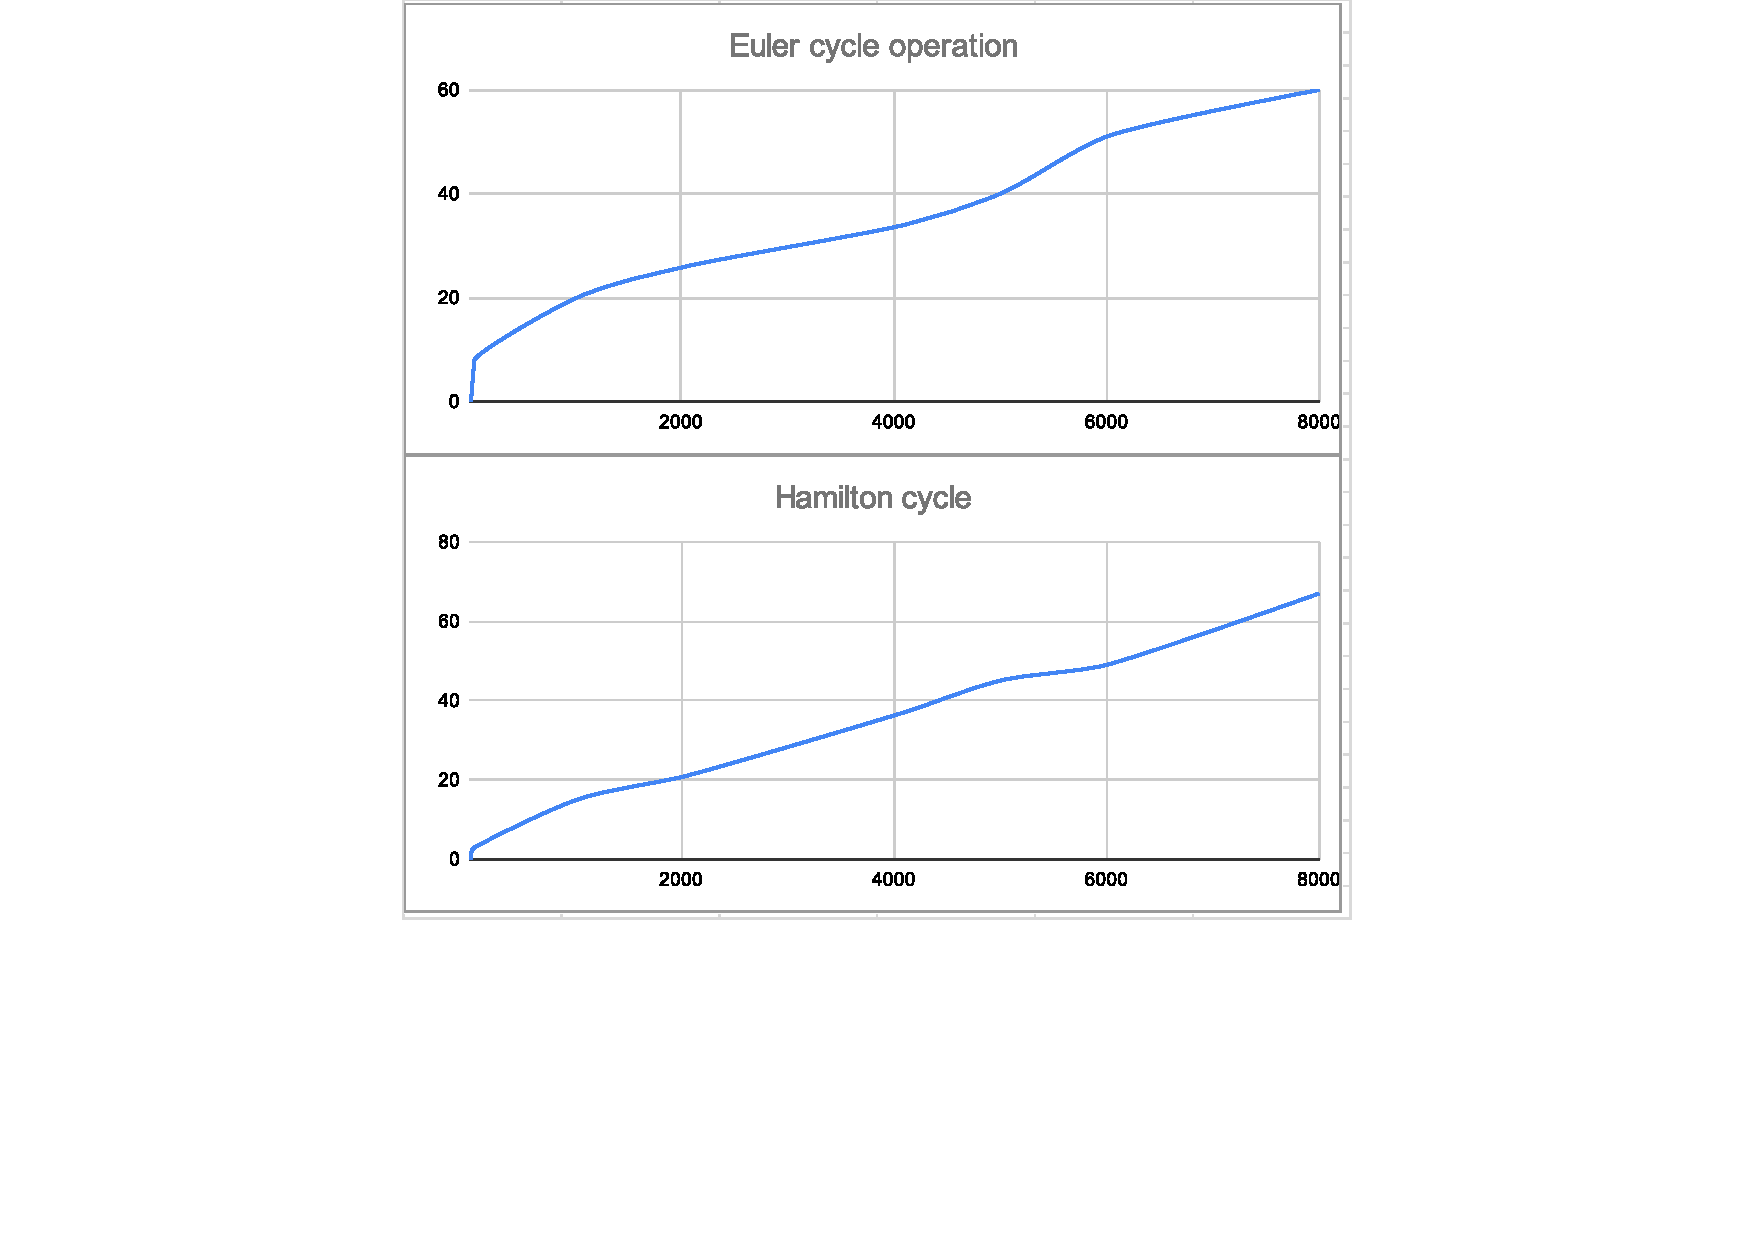
\includegraphics[width=\linewidth]{wykres_liniowy_0.pdf}

\end{center}

\subsection{Skala logarytmiczna t(ms): }

\begin{center}

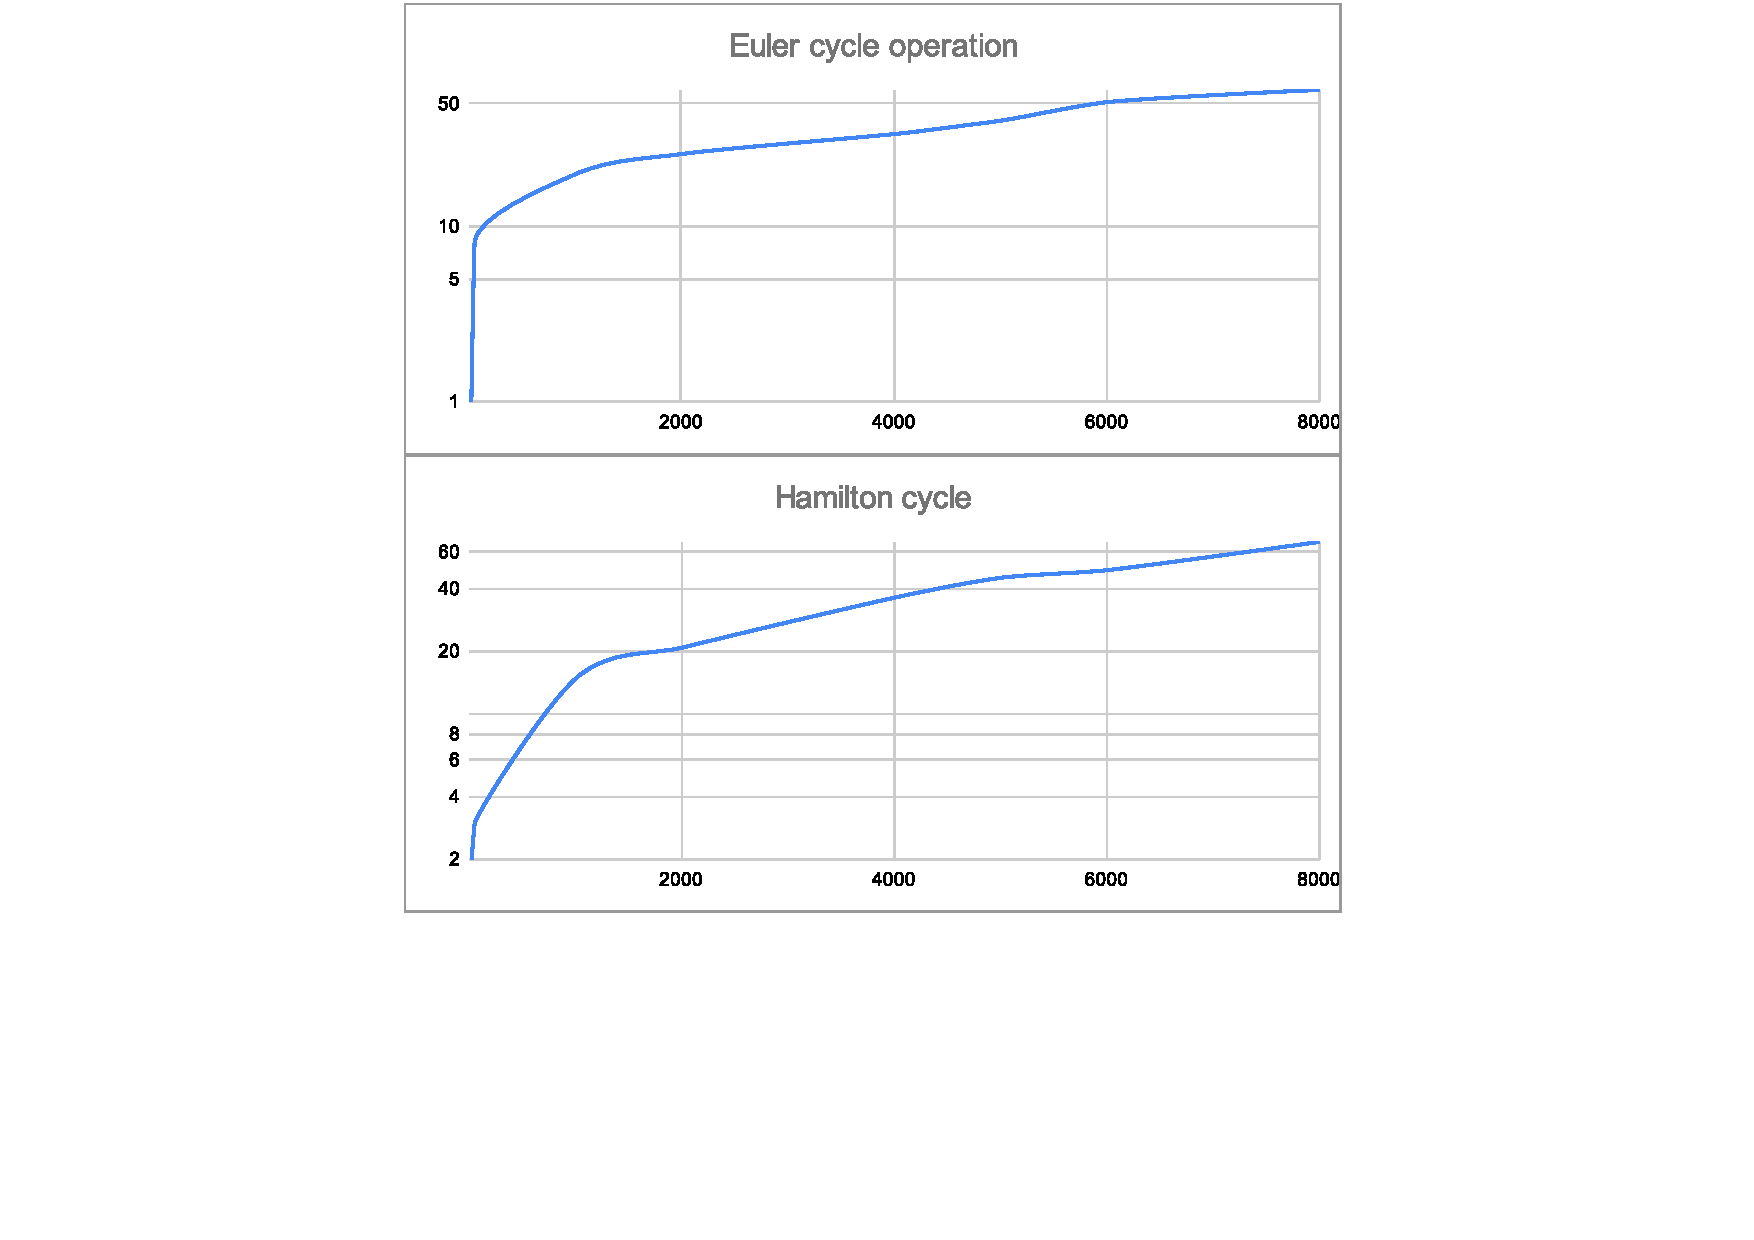
\includegraphics[width=\linewidth]{wykres_logarytmiczny_0.pdf}

\end{center}

\section{Wykresy zależności: (dla grafów nie hamiltonowskich o nasyceniu 50) $ t = f(n) $}

\subsection{Skala liniowa t(ms): }

\begin{center}

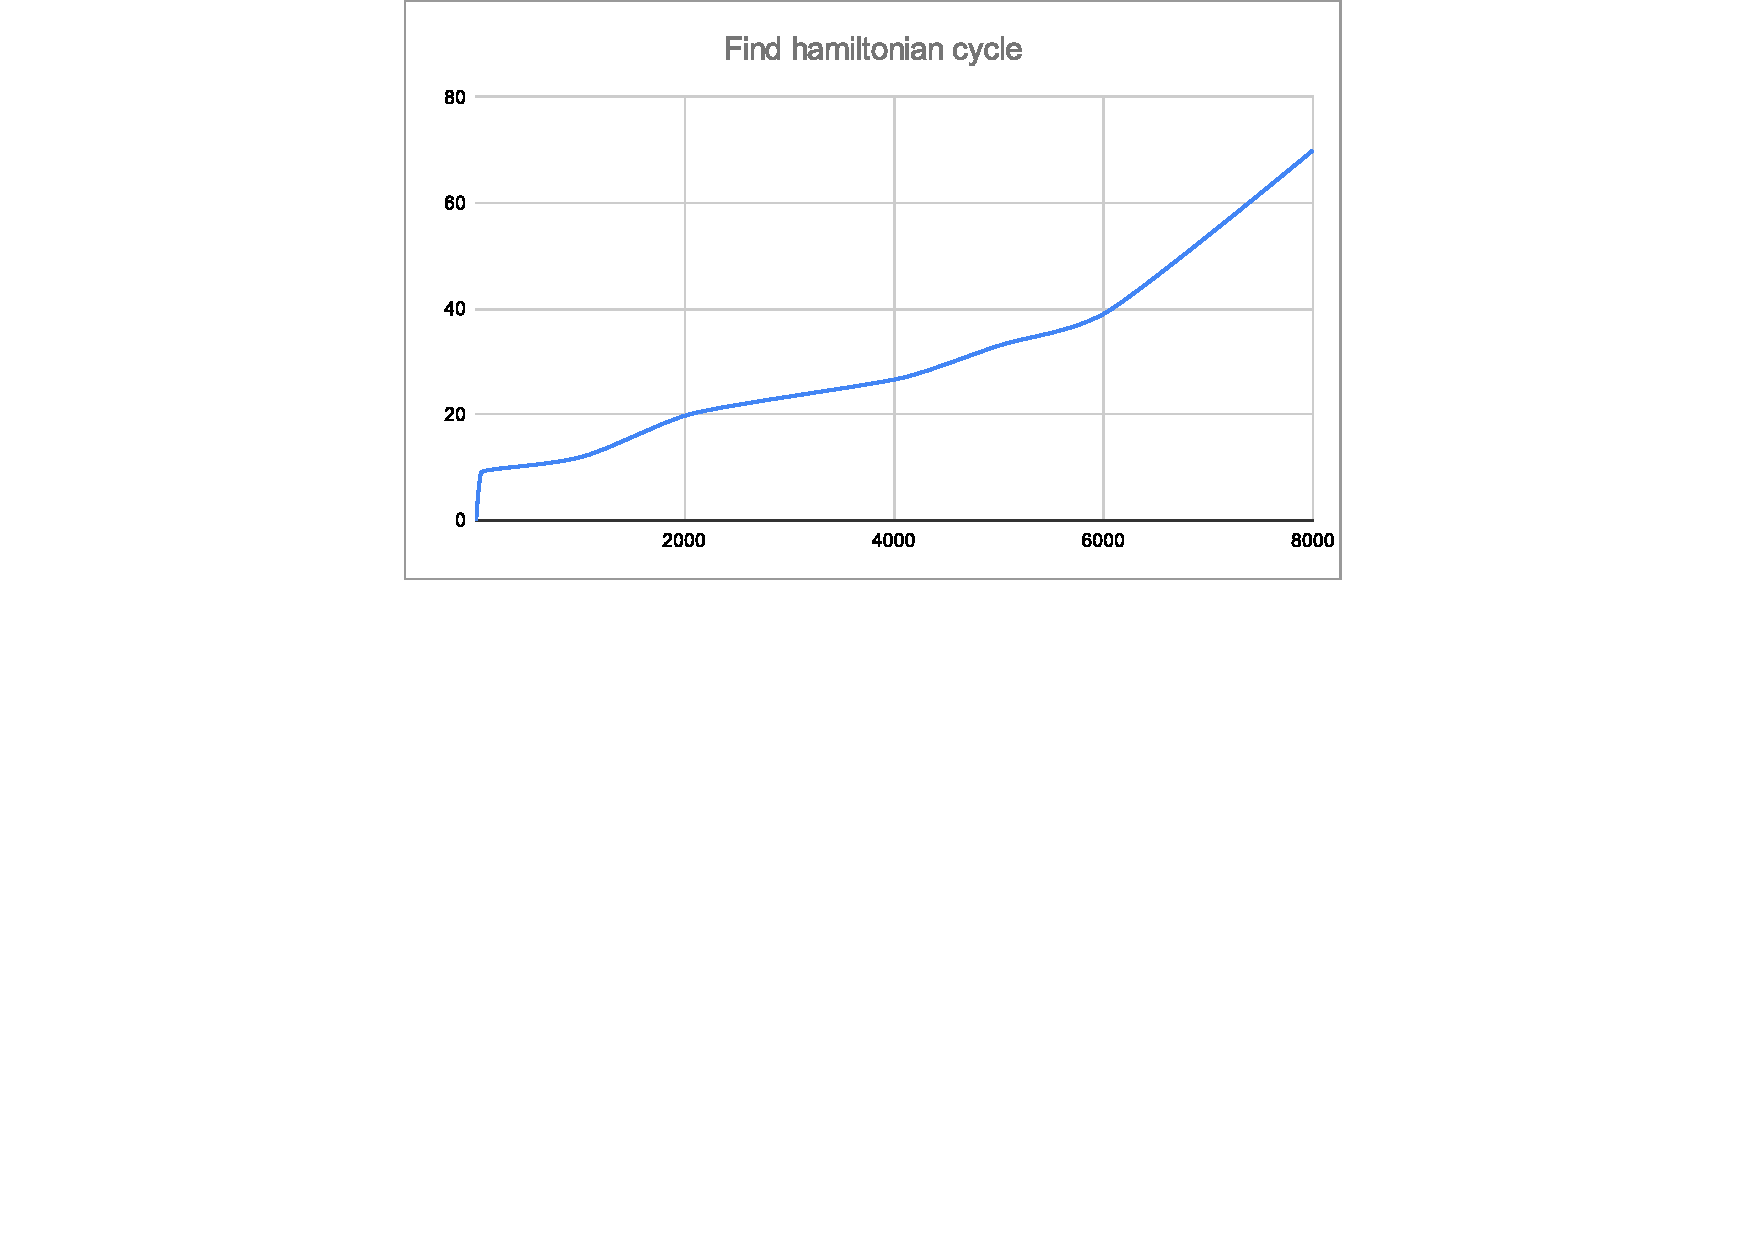
\includegraphics[width=\linewidth]{wykres_liniowy_1.pdf}

\end{center}

\subsection{Skala logarytmiczna t(ms): }

\begin{center}

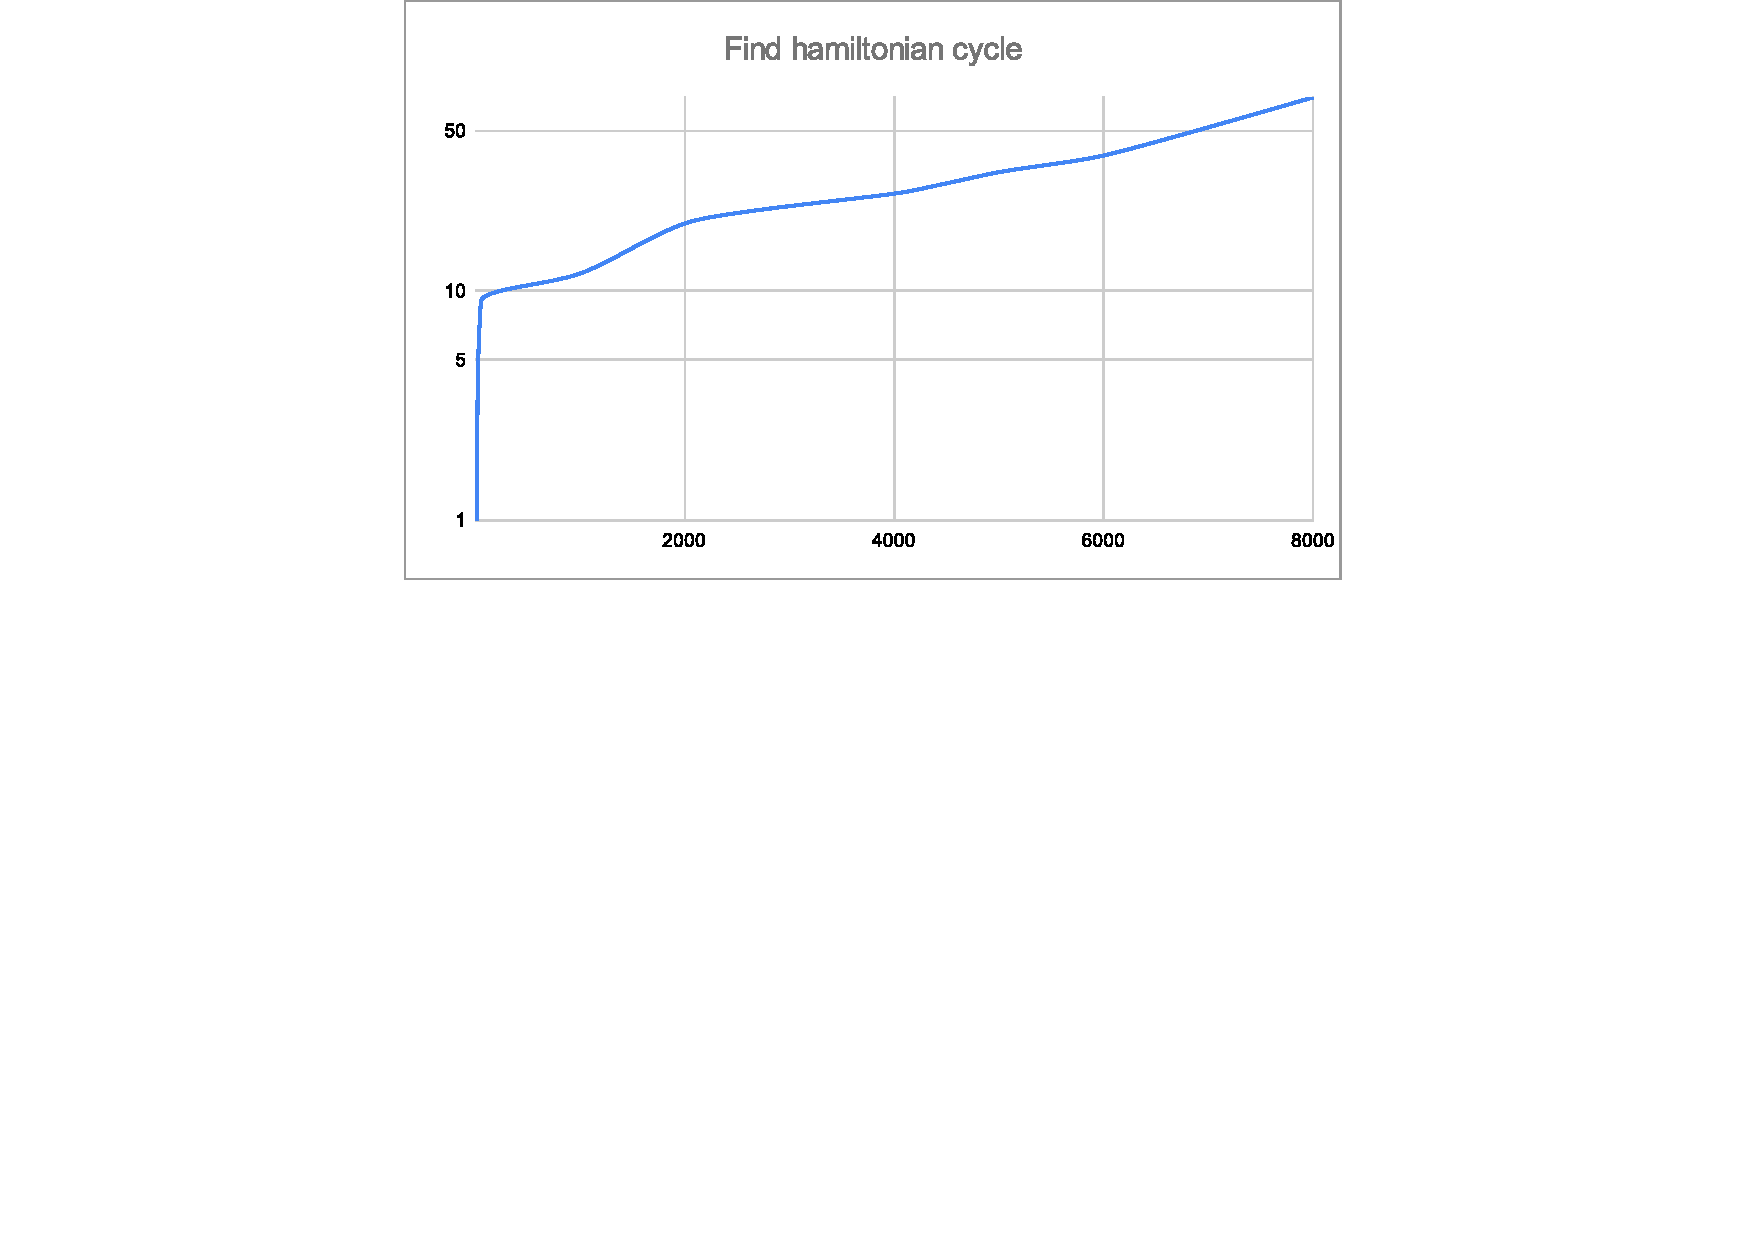
\includegraphics[width=\linewidth]{wykres_logarytmiczy_1.pdf}

\end{center}

\section{Podsumowanie: }

Nauczyłem sie

\begin{enumerate}

	\item
	      Generować grafy.
	\item
		  Implementowac algorytmy ktore operuja na tych strukturach.
	\item
		  O grafach jako strukturach danych.
	\item
		  Jak zaimplementować algorytmy BFS i DFS.
	\item
		  Jak znajdowac krawedzie w grafach.
    \item
    	      Wypisywania na ekran.
  	\item
  		  Implementować algorytmy grafowe dla różnych reprezentacji maszynowych grafów.

\end{enumerate}

\tableofcontents

\end{document}